\documentclass[a4paper]{article}
\usepackage[T1]{fontenc}
\usepackage[utf8x]{inputenc}
\usepackage[margin=1.1in]{geometry}
\usepackage[english]{babel}
\usepackage{graphicx}
\usepackage{parskip}
\usepackage{float}
\usepackage[procnames]{listings}
\usepackage{color}

\definecolor{keywords}{RGB}{255,0,90}
\definecolor{comments}{RGB}{0,0,113}
\definecolor{red}{RGB}{160,0,0}
\definecolor{green}{RGB}{0,150,0}

\lstset{language=Python, 
		basicstyle=\ttfamily\small, 
		keywordstyle=\color{keywords},
		commentstyle=\color{comments},
		stringstyle=\color{red},
		numbers=left,
		stepnumber=1,	
		showstringspaces=false,
		breaklines=true,
		breakatwhitespace=false,	
		identifierstyle=\color{green},
		procnamekeys={def,class}}

\usepackage{setspace} % increase interline spacing slightly
\setstretch{1.1}

\title{
	Big Data Analytics \\
	Lab 01 - Hadoop MapReduce in the cloud}
\author{
	Damien Rochat, Dorian Magnin, and Nelson Rocha \\
	Master of Science in Engineering \\
	University of Applied Sciences and Arts Western Switzerland}
\date{\today}

\begin{document}
	\maketitle
	
	\section{Task 2: Using Elastic MapReduce}

	\subsection{EMR console summary}
	\begin{figure}[H]
		\centering
		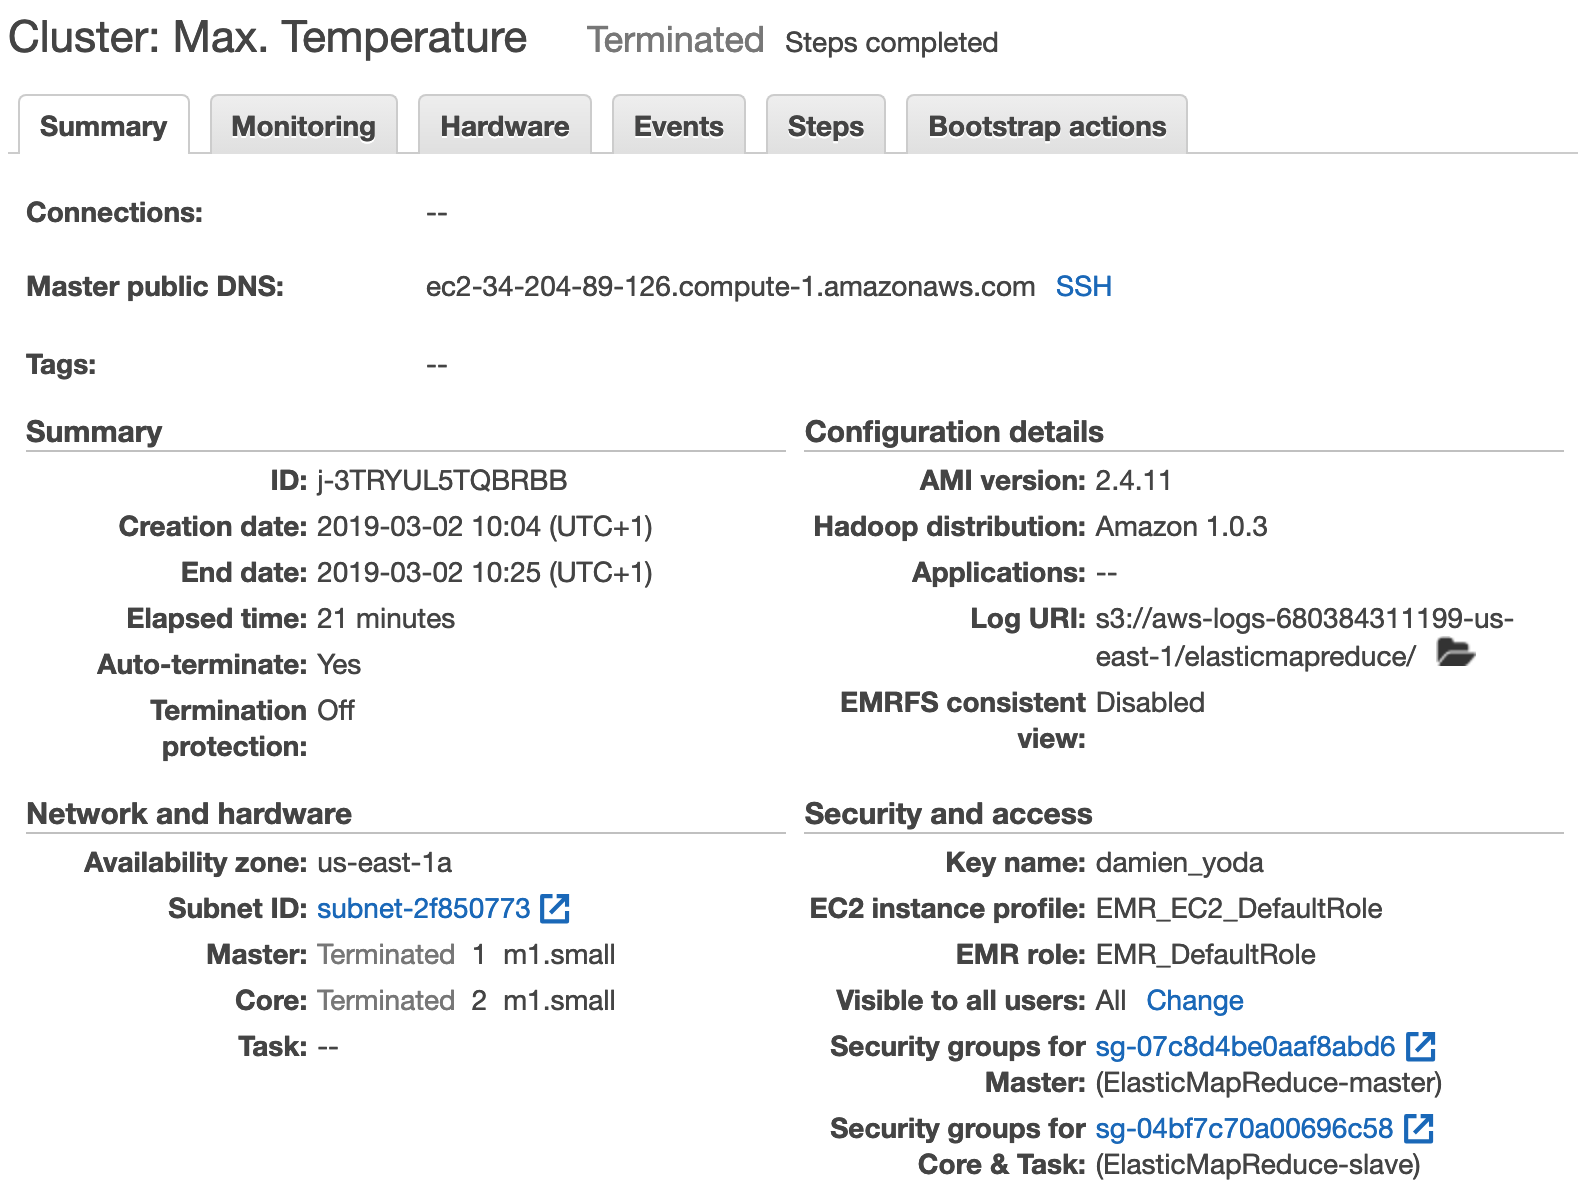
\includegraphics[width=\columnwidth]{ex02/emr_console.png}
		\caption{Elastic MapReduce summary}
		\label{fig:emr-summary}
	\end{figure}

	\subsection{Max temperature chart}
	\begin{figure}[H]
		\centering
		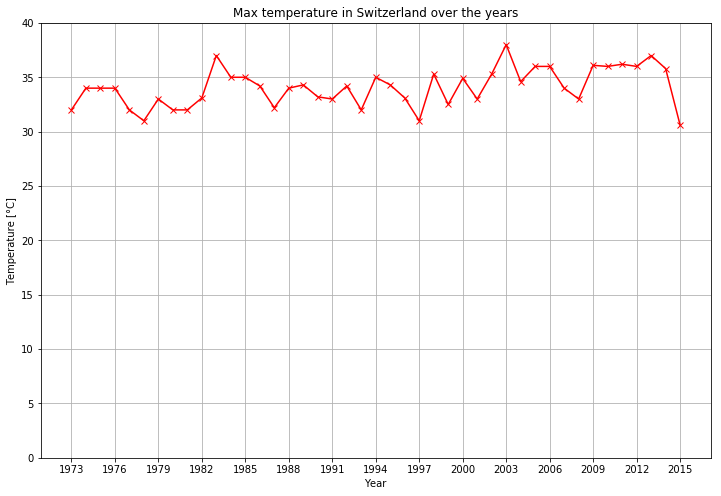
\includegraphics[width=\columnwidth]{ex02/max_temperature_chart.png}
		\caption{Max temperature chart}
		\label{fig:max-temp-chart}
	\end{figure}

	The overall highest recorded temperature is of 38.0 °C in 2003, year of the European heat wave.

	\subsection{EC2 instances}
	We used 3 m1.small instances (1 master and 2 cores). \\
	For each one, the price of the on-demand EC2 is \$0.044 + \$0.011 for the EMR per hour.
	Our cluster ran during 21 minutes.
	
	The total cost is of \$0.0693 ($(\$0.055+\$0.011)*3*0.35 = \$0.0693$).
	
	\subsection{EMR job}
	From the job log file, the Mappers processed \textbf{2'831'380} input records (MAP\_INPUT\_RECORDS) and produced \textbf{2'821'078} records (MAP\_OUTPUT\_RECORDS). \\
	The Reducers processed \textbf{2'821'078} input records (REDUCE\_INPUT\_RECORDS) and produced \textbf{43} records (REDUCE\_OUTPUT\_RECORDS).

	\pagebreak

	\section{Task 3: Writing a MapReduce program}

	\subsection{Source code}

	\subsubsection{Mapper}
	\lstinputlisting[
		label={lst:max-temp-map},
		caption={max\_temperature\_map.py source code},
		captionpos=b,
		language=Python]{ex03/count_temperature_map_optimized.py}

	\subsubsection{Reducer}
	\lstinputlisting[
		label={lst:max-temp-reduce},
		caption={max\_temperature\_reduce.py source code},
		captionpos=b,
		language=Python]{ex03/count_temperature_reduce_optimized.py}

	We also tried a non-optimized version of the code (without "In-Mapper combining") and obtained a time difference of 3 minutes (10 minutes instead of 7 minutes) on the EMR step duration.

	\subsection{Stats}
	How often does the temperature 22 degrees celsius occur? \textbf{56'530 times}

	What is the lowest and highest temperature occuring? \textbf{min: -25 °C, max: 38 °C}

	Which temperature occurs most often? \textbf{13 °C} with \textbf{114'613 occurences}

	\subsection{Histogram}
	\begin{figure}[H]
		\centering
		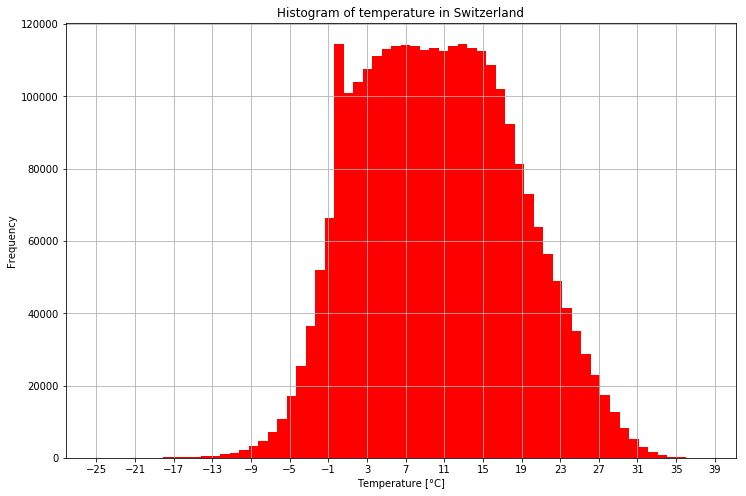
\includegraphics[width=\columnwidth]{ex03/temperature_histogram.png}
		\caption{Histogram of temperature in Switzerland}
		\label{fig:swiss-temp-histogram}
	\end{figure}

\end{document}
